\chapter{Local Context}\label{ch:localcontext}
    Il riconoscimento dei diagrammi viene effettuato in base al \textit{Local Context}, presentato nei paper~\cite{localcontext_recognition},~\cite{extending_localcontext} e~\cite{localcontext}.
    \newline
    Nel paper \textit{Local context-based recognition of sketched diagrams} \cite{localcontext_recognition}, il Local Context viene presentato come una nuova metodologia mirata alla creazione e all'implementazione di un framework\footnote{\textit{`Un framework, in generale, include software di supporto, librerie, un linguaggio per gli script e altri software che possono aiutare a mettere insieme le varie componenti di un progetto.`, \cite{framework}}} per il riconoscimento e l'interpretazoine dei diagrammi. Nello specifico, i diagrammi possono contenere differenti elementi grafici quali simboli, connettori e testo. Una volta che i simboli sono stati identificati, il riconoscimento procede identificando il contesto locale di ogni simbolo.
    Il Local Context ha due diverse specifiche: sintattiche e semantiche.
    \section{Sintassi}
        Sempre in~\cite{localcontext_recognition}, viene definita la specifica sintattica di un linguaggio visuale.
        In particolare, usando il contesto locale, la specificazione della sintassi di un linguaggio visivo consiste di svariati elementi quali:
        \begin{itemize}
            \item Definizione dei simboli (token) che compongono il linguaggio visuale:
            \begin{itemize}
                \item Definizione dell'apparenza ''fisica'' dei simboli (ad esempio forma, colore, ecc.);
                \item Definizione degli attributi del simbolo della loro forma e del loro aspetto (ad esempio punti/area d'attaccamento, ecc);
                \item Definizione dei vincoli locali al simbolo riguardanti gli attributi (ad esempio il numero di connessioni permesse ad un punto d'attaccamento, ecc.).
            \end{itemize}
            \item Definizione delle relazioni/connettori e i loro vincoli locali;
            \item Dichiarazione di vincoli al livello del diagramma (ad esempio numero di occorrenze ammisibili di un simbolo, se i simboli e i connettori devono formare un grafo connesso);
            \item Una grammatica per definire ulteriori vincoli di sintassi del linguaggio (quando necessario).
        \end{itemize}

        \begin{table}[htbp]
            \centering
            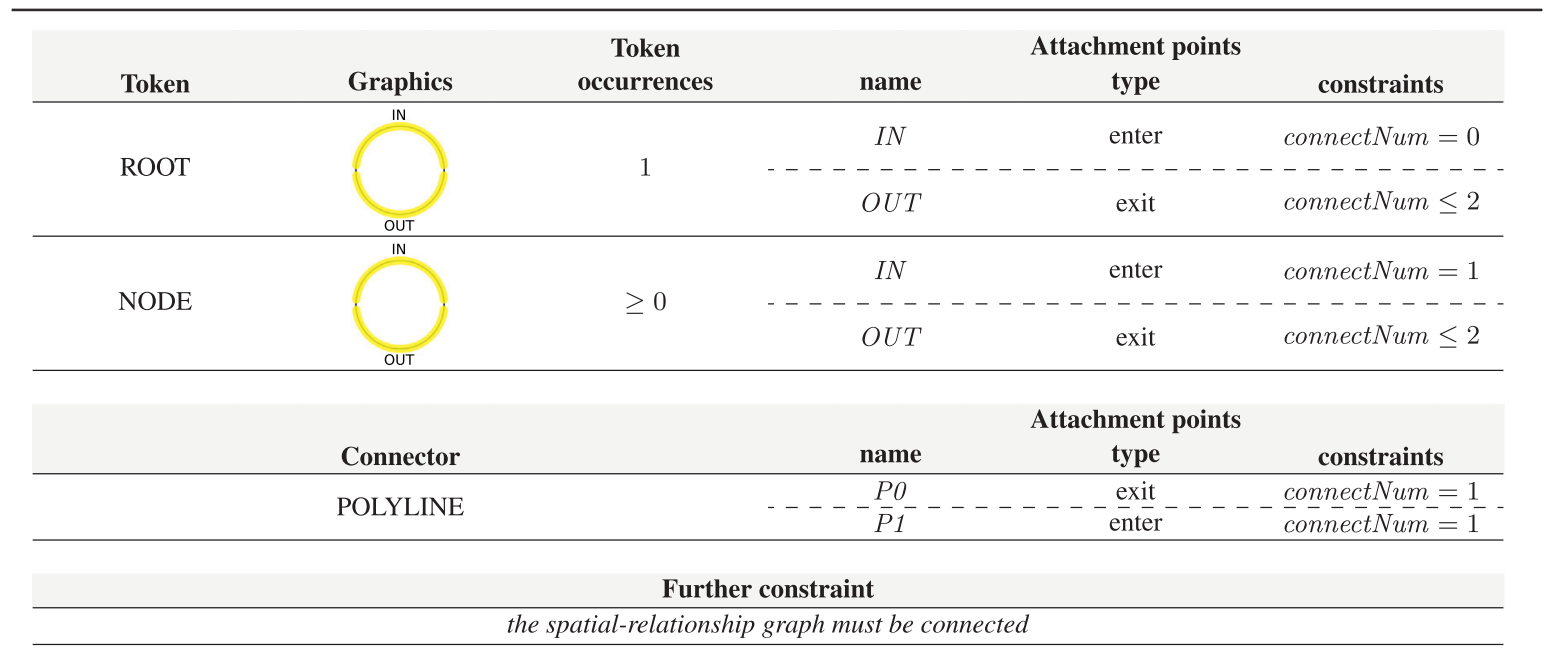
\includegraphics[scale=0.35]{Figure/elem_specification.PNG}
            \caption{Specifica di un linguaggio, nel particolare di un Albero}
            \label{tab:elem_specification}
        \end{table}
        \noindent
        Facendo riferimento alla tabella~\ref{tab:elem_specification}, ovvero la specifica di un linguaggio che identifica un Albero, possiamo notare che ogni riga identifica un simbolo (o token) e che ogni riga è composta da sei colonne, le prime tre sono indirizzate al livello del simbolo e le restanti tre colonne indicano i vincoli per gli attachment points:
        \begin{itemize}
            \item \textbf{Token}: indica il nome dell'elemento;
            \item \textbf{Graphics}: rappresentazione grafica dell'elemento e rappresentazione dei punti d'attaccamento evidenziati in giallo;
            \item \textbf{Token occurences}: numero di occorrenze ammisibile per quel simbolo;
            \item \textbf{name}: può essere composta da più righe ed indica i nomi dei punti d'attaccamento;
            \item \textbf{type}: la tipologia di AP\footnote{Punti d'attaccamento.}, un tipo di punto di attaccamento può avere più nomi;
            \item \textbf{constraints}: i vincoli al livello dei punti d'attaccamento, \textit{connectNum} indica il numero di archi incidenti a quel determinato AP.
        \end{itemize}
        I vincoli al livello della sentenza sono riportati nell'ultima riga. Una parte della formalizzazione della tabella \ref{tab:elem_specification} in formato XML è mostrata nello snippet di codice \ref{lst:xml_elem_specification}, l'intera specifica è consultabile nell'appendice \ref{appendix:xml_definition}.

        \lstinputlisting[caption={\textbf{Frammento della definizione in formato XML di un linguaggio, nel particolare la specifica per il simbolo \textit{root} (o radice).}},label={lst:xml_elem_specification},language=Xml, firstline=2, lastline=7]{SourceCode/tree_specific.xml}

        \noindent
        Nel paper~\cite{extending_localcontext}, viene esteso il concetto della specifica semantica esposta in~\cite{localcontext_recognition} aggiugendo nuove caratteristiche alla specifica del contesto locale per permettere la specifica di linguaggi visuale più complessi quali diagrammi entità-relazione, use case diagrams e class diagram. In più viene presentato un tool (LoCoMoTiVE, specificato nel paragrafo 2.2) che implementa il framework \textit{Local Context}.
        \newline
        Le principali caratteristiche aggiunte sono tre:
        \begin{itemize}
            \item La definizione di vincoli al livello del simbolo può coinvolgere più di un area di attaccamento di un simbolo/connettore al contrario di vincolare aree d'attaccamento individuali;
            \item La definizione di un vincolo per limitare auto-cicli di un connettore;
            \item Assegnazione di più tipi alle aree di attaccamento.
        \end{itemize}

    \section{Semantica}
        In \cite{localcontext} viene esteso il framework definendo una nuova tecnica per una traduzione semantica del liguaggio visuale basata sul contesto locale. Questa tecnica usa delle esspressioni simili a queli di XPath, chiamate SGPath, illustrate nel dettaglio nel capitolo 5.
        \newline
        Per consentire la traduzione semantica di un linguaggio visuale è stata descritta una definizione semantica basata sul contesto locale o \textit{LCSD}\footnote{Local Context-based Semantic Definition} e il suo algoritmo per valutarla. L'LCSD consiste di una sequenza di regole semantiche una per ogni elemento del linguaggio. Ogni regola calcola una proprietà attraverso delle procedure che fanno uso degli SGPath o esegue un'azione che dipende dalla proprietà e gli attributi. Ogni proprietà può avere una post-condizione.
        \newline
        Attraverso le post-condizioni, una LCSD può dare una definizione migliore della struttura sintattica; attraverso le azioni restituisce una traduzione delle sentenze. Un'azione dipende da proprietà e attributi.
        \begin{table}[htbp]
            \centering
            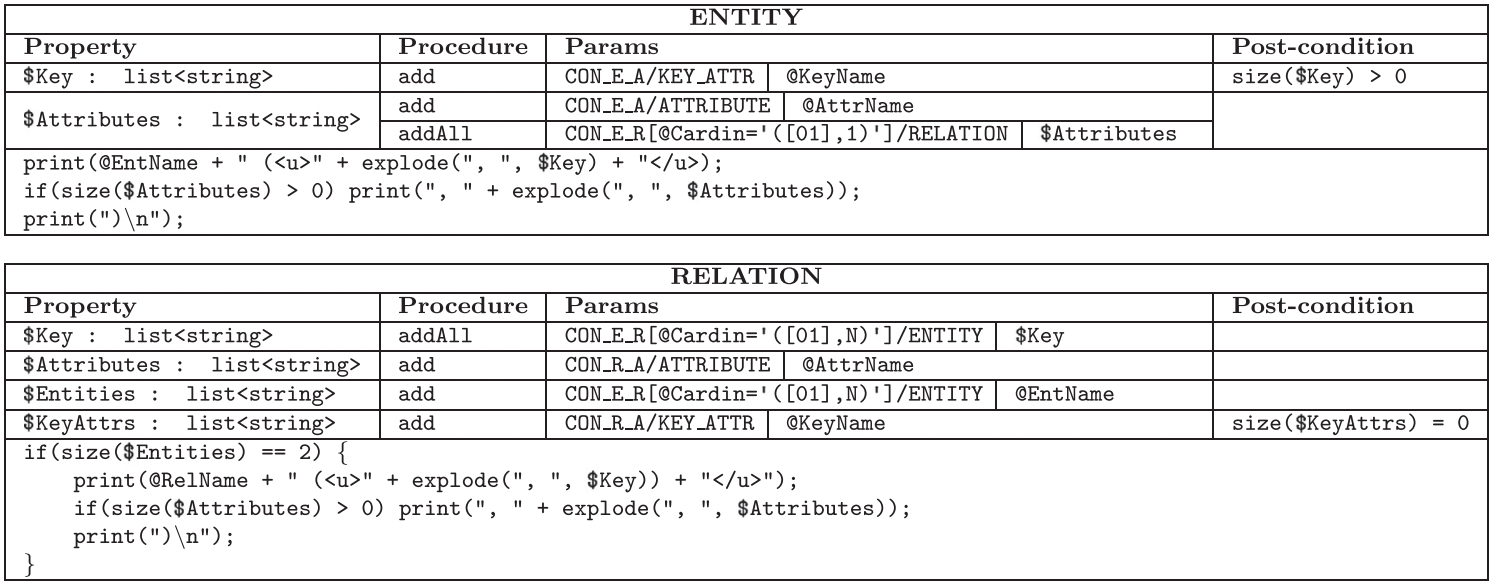
\includegraphics[scale=0.37]{Figure/semantic_specification.PNG}
            \caption{Specifica LCSD di un diagramma ER, costruita sulla specifica sintattica.}
            \label{tab:semantic_specification}
        \end{table}
        \newline
        La tabella \ref{tab:semantic_specification} mostra una specifica semantica di un diagramma ER\footnote{Entità Relazione.}. Ogni tabella fornisce le regole semantiche di un elemento, in questo caso per i simboli ENTITY e RELATION, rispettivamente. Ogni riga della specifica è composta dai seguenti elementi:
        \begin{itemize}
            \item \textbf{Property}: indica il nome della proprietà (preceduta dal carattere \$) e il tipo.
            \item \textbf{Procedure}: indica il nome della procedura da utilizzare per assegnare/modifcare il valore di una proprietà, ogni proprietà può avere più procedure.
            \item \textbf{Params}: i parametri da utilizzare nella procedura. Il primo parametro è un SGPath, il secondo parametro è il nome della proprietà dove leggere le informazioni del/i simbolo/i raggiungibile/i con quel percorso.
            \item \textbf{Post-condition}: la post-condizione che deve essere rispettata al termine dell'esecuzione della procedura. 
        \end{itemize}
        L'ultima colonna indica l'azione da eseguire. A differenza dell'attuale implementazione, TiVeJS può eseguire anche azioni parziali, ovvero posizionata tra le proprietà e non dopo le proprietà.
        \newline
        \begin{figure}[htbp]
            \centering
            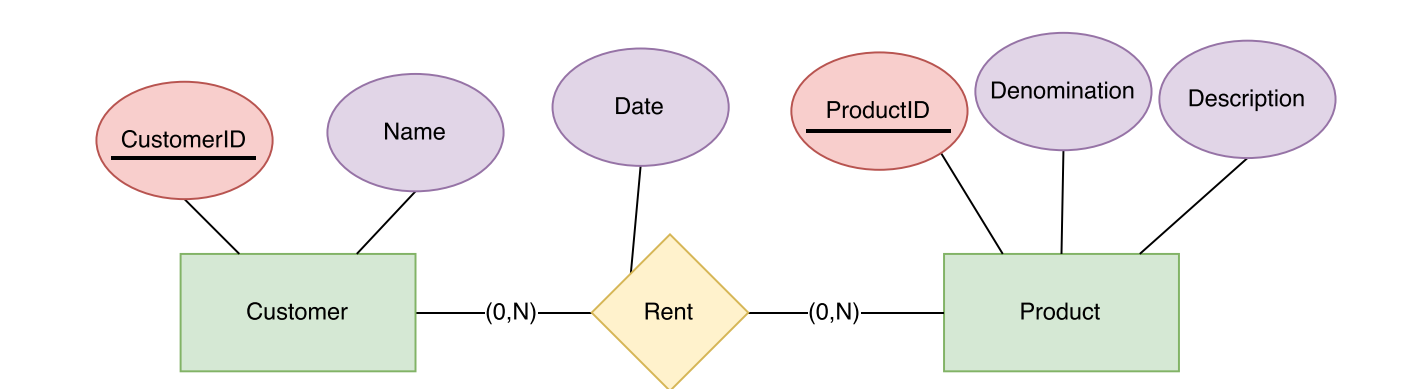
\includegraphics[scale=0.4]{Figure/er_diagram.PNG}
            \caption{Diagramma ER}
            \label{fig:er_diagram}
        \end{figure}
        In questo caso, applicando le regole semantiche definite nella tabella \ref{tab:semantic_specification} al diagramma \ref{fig:er_diagram} produrrà la seguente traduzione semantica:
        \begin{quotation}
            \noindent
            Customer (\underline{CustomerID}, Name) \newline
            Product (\underline{ProductID}, Denomination, Description) \newline
            Rent (\underline{CustomerID, ProductID}, Date)
        \end{quotation}
        Tutti i dettagli implementativi saranno illustrati nel prossimo capitolo.